\beginsong{Was wollen wir trinken}[wuw={Bots}, pfii={136}, pfiii={32}]

\markboth{\songtitle}{\songtitle}

\beginverse
\endverse

\centering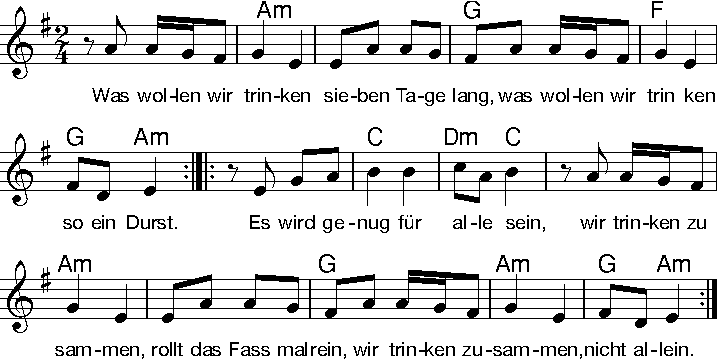
\includegraphics[width=1\textwidth]{Noten/Lied093.pdf}

\beginverse
\lrep Dann wollen wir \[Am]schaffen , 7 Tage \[G]lang,
dann wollen wir \[F]schaffen, \[G]komm fass \[Am]an. \rrep
\lrep Und das wird \[C]keine \[Dm]Placke\[C]rei,
wir schaffen zu\[Am]sammen, 7 Tage \[G]lang,
wir schaffen zu\[F]sammen, \[G]nicht al\[Am]lein. \rrep
\endverse
\beginverse

\lrep Jetzt müssen wir ^streiten, keiner weiß wie ^lang,
ja, für ein ^Leben ^ohne ^Zwang. \rrep
\lrep Dann kriegt der ^Frust uns ^nicht mehr ^klein,
wir halten zu^sammen, keiner kämpft al^lein,
wir gehen zu^sammen, ^nicht al^lein. \rrep
\endverse
\beginverse
 
\lrep Dann wollen wir \[Am]trinken, 7 Tage \[G]lang,
dann wollen wir \[F]trinken, \[G]wir haben \[Am]Durst.\rrep
\lrep Es ist ge\[C]nug für \[F]alle \[C]da,
wir trinken zu\[Am]sammen, roll das Fass mal \[G]rein,
wir trinken zu\[F]sammen, \[G]nicht al\[Am]lein. \rrep
\endverse

\endsong

\beginscripture{}
Die Melodie zu diesem Lied taucht zum ersten Mal 1929 auf. Ab den 1970ern wird es immer wieder mit verschieden Texten versehen und feiert mehrere Erfolge.
\endscripture

\begin{intersong}

\end{intersong}